

Todas as aplicações desenvolvidas são inicializadas da mesma forma:
basta executar o módulo ``main'' de cada pacote. Para funcionar, a
aplicação da simulação deve ser chamada primeiro. As telas da
aplicação de visualização e das mensagens do simulador podem ser
vistas nas figuras \ref{pic_viewer} e \ref{pic_sim}, respectivamente.

\begin{figure}[H]
  \caption{\label{pic_viewer} Tela da interface de visualização, após
    aumento de $30\%$ na vazão de vapor}
  \centering
  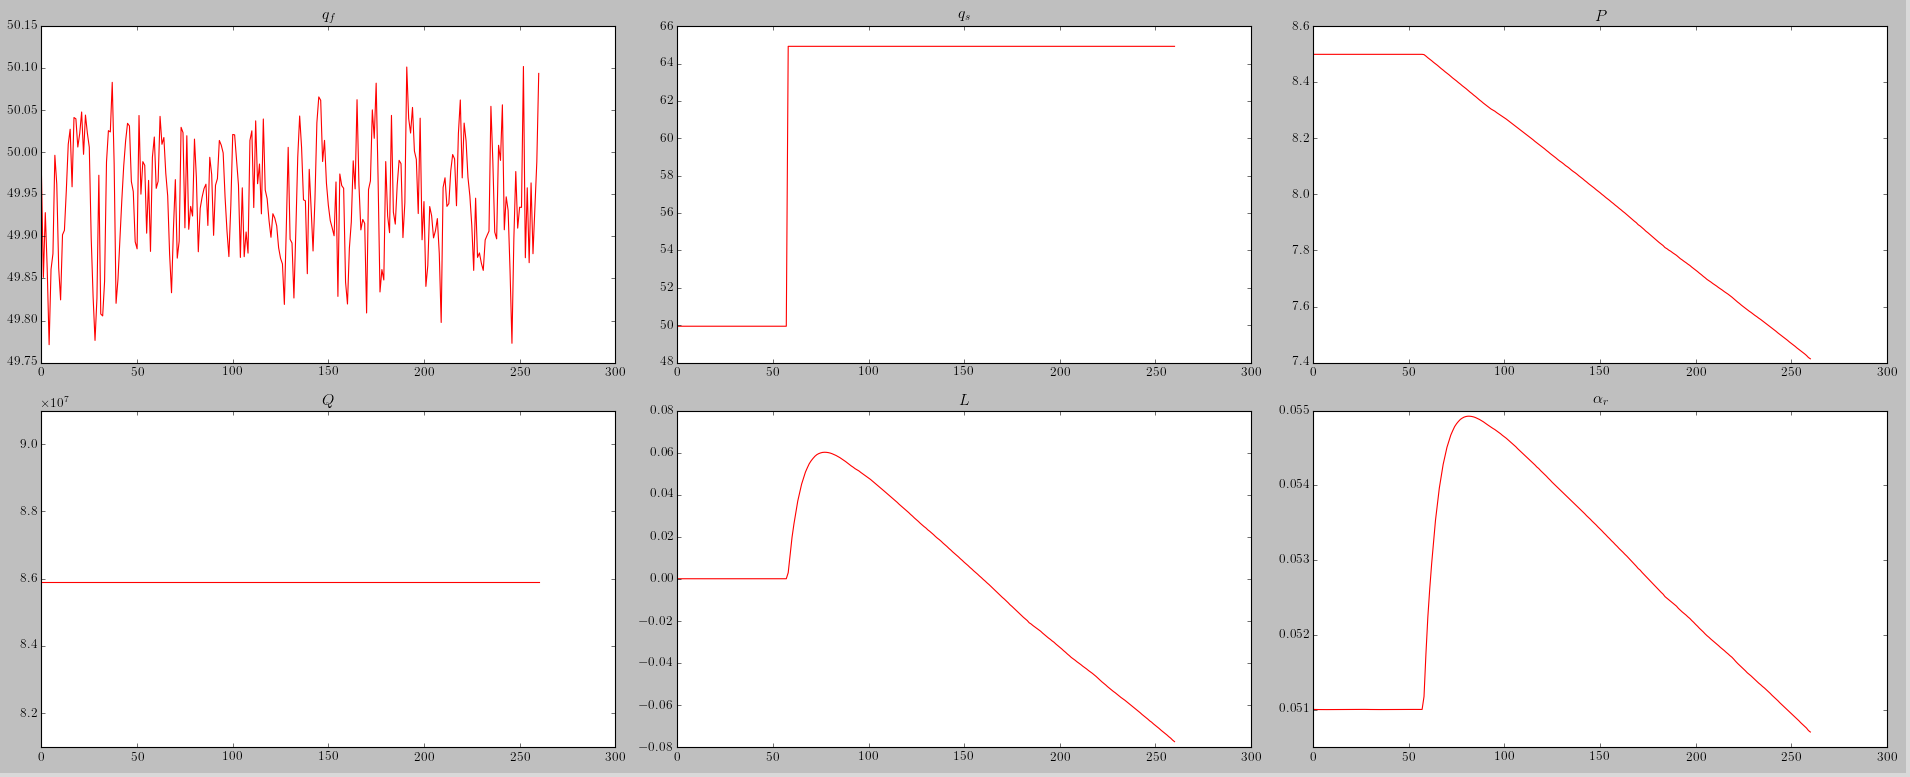
\includegraphics[scale=0.25]{img/pic_viewer.png}
\end{figure}

\begin{figure}[H]
  \caption{\label{pic_sim} Tela do simulador enviando e recebendo
    mensagens}
  \begin{center}
    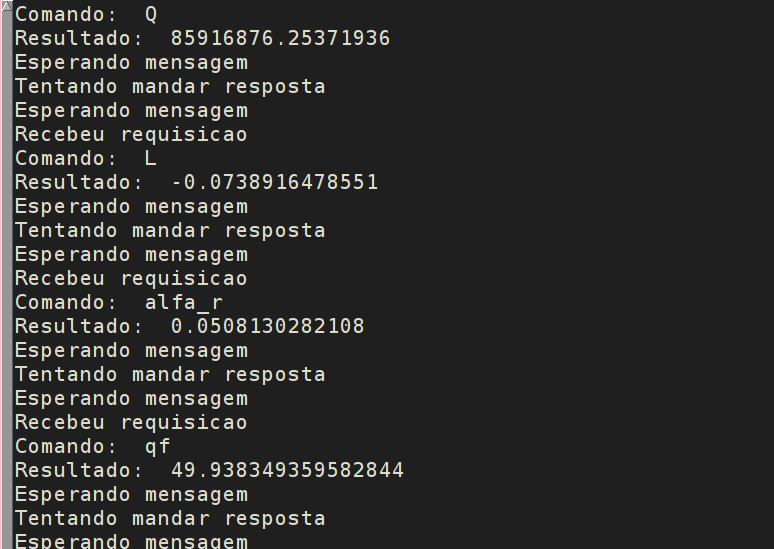
\includegraphics[scale=0.3]{img/pic_sim.png}
  \end{center}
\end{figure}

Na figura \ref{pic_viewer_controllers}, pode-se ver a tela da
interface quando o sistema responde a um aumento de $30\%$ na vazão de
vapor com os controladores ligados. Isso mostra a independência das
aplicações, podendo ativar ou desativar cada uma separadamente, mesmo
com o sistema funcionando.

\begin{figure}[H]
  \caption{\label{pic_viewer_controllers} Tela da interface de
    visualização após aumento de $30\%$ na vazão de vapor, com
    controladores em funcionamento}
  \centering
  \subbottom[\label{pic_viewer_controllers:pressao}Somente controle da
    pressão]{
    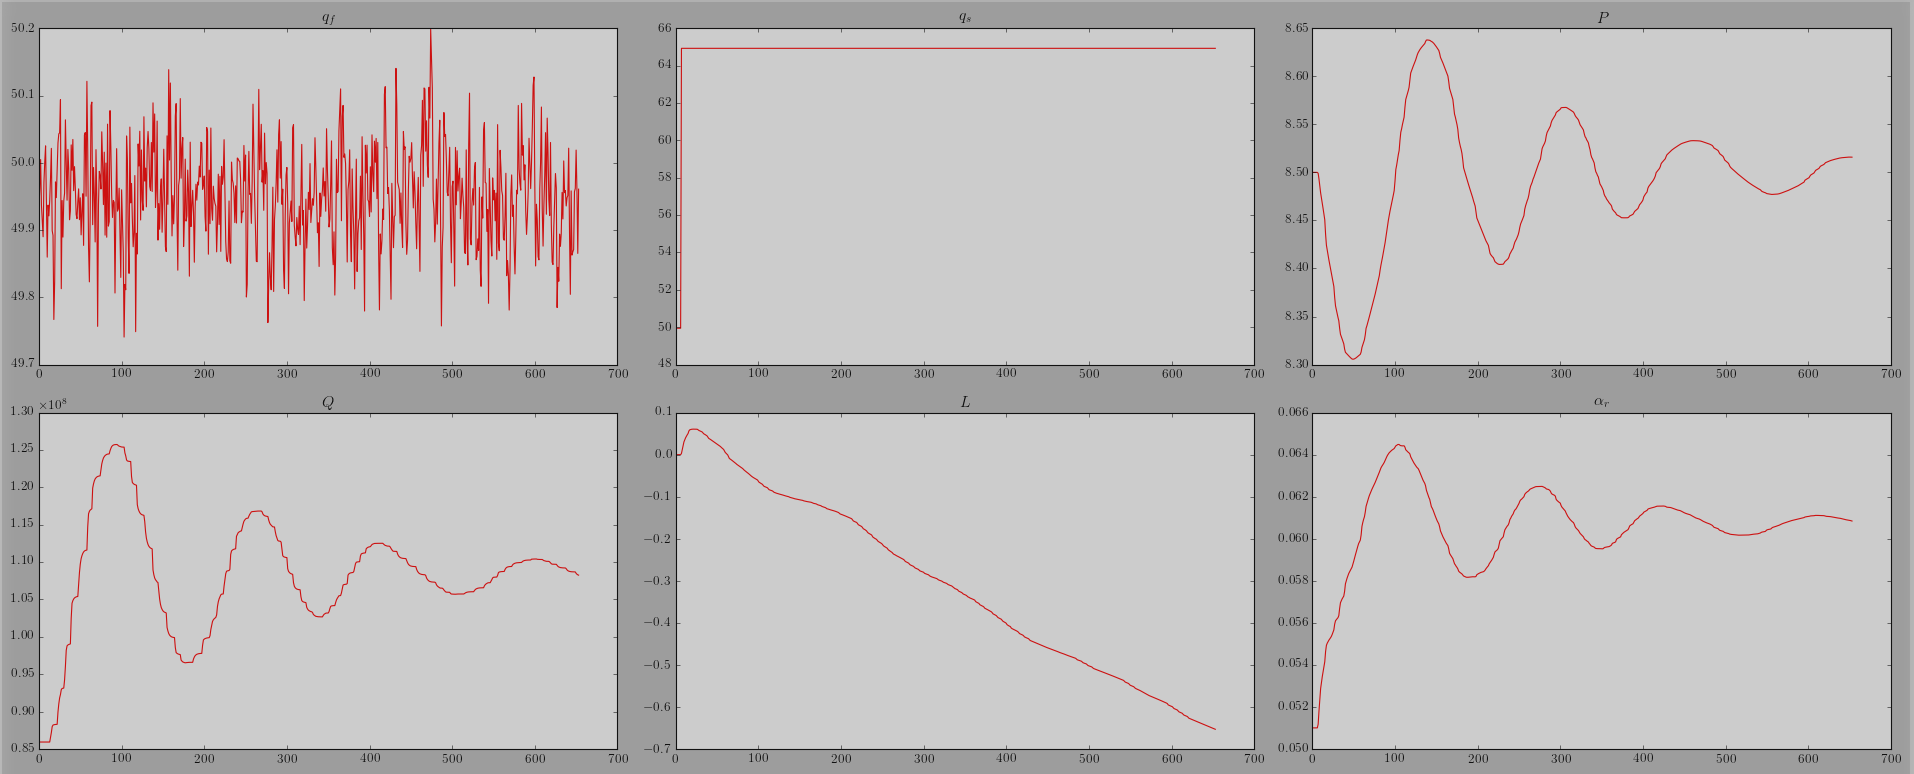
\includegraphics[scale=.25]{img/viewer_contr_pressao.png}}
  \subbottom[\label{pic_viewer_controllers:completo}Controle de
    pressão e nível]{
    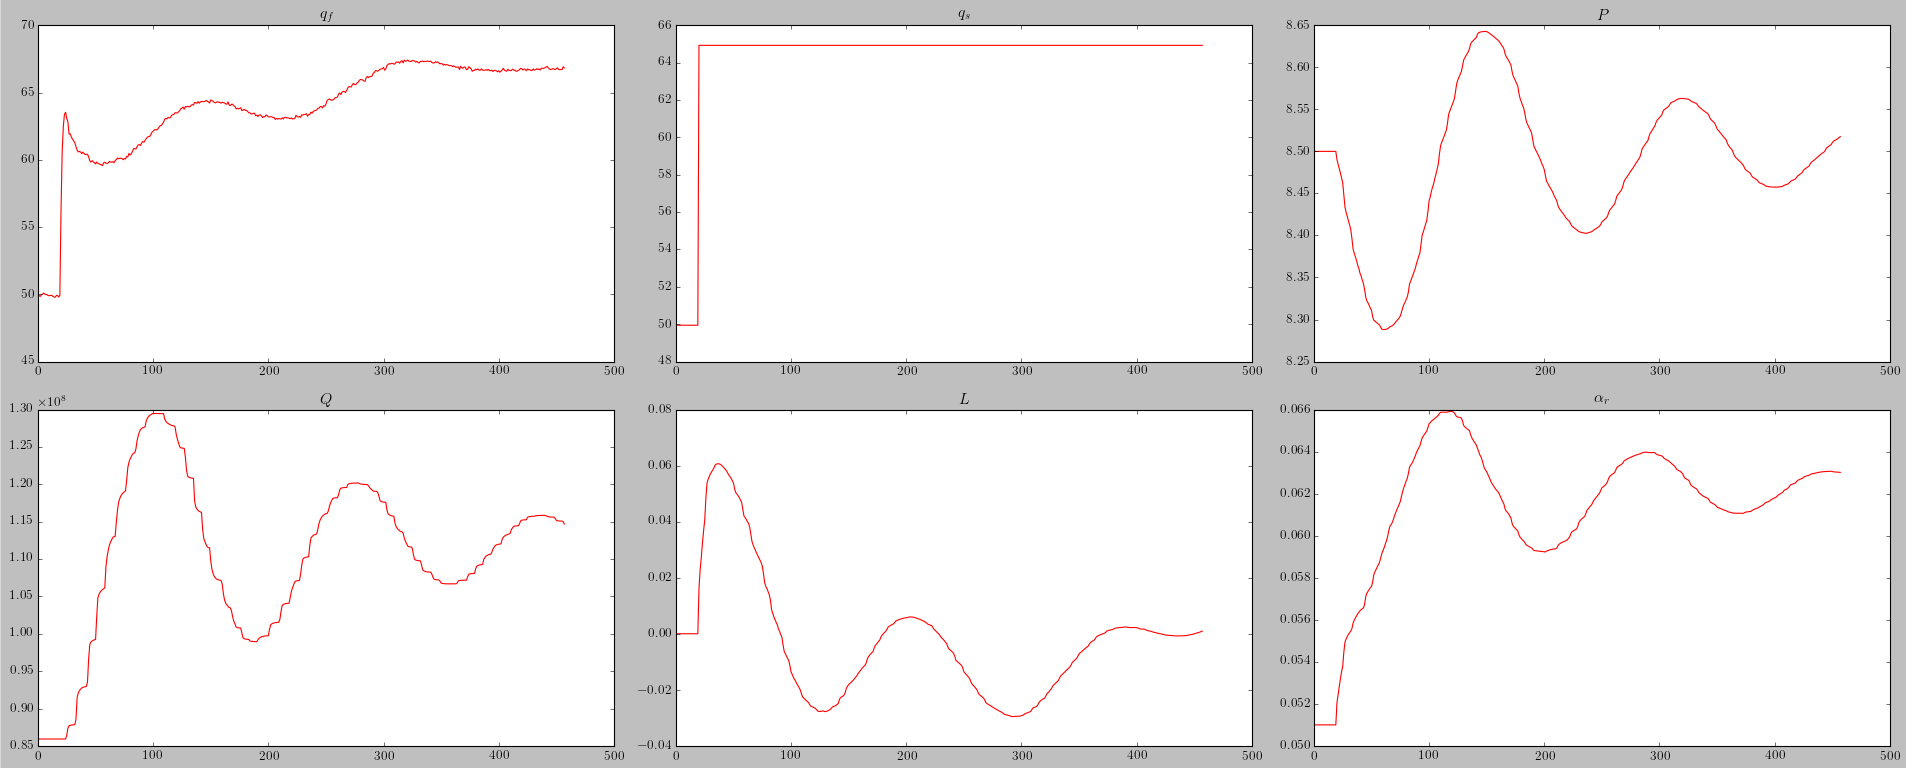
\includegraphics[scale=.25]{img/viewer_controlado.png}}

\end{figure}

Pode-se ver que, apesar de não serem ideais, os controladores são
estáveis, conseguindo ajustar os parâmetros da caldeira corretamente.

Pode-se também usar o console do Python para enviar mensagens usando a
classe de interface cliente, controlando manualmente a planta. A
figura \ref{pic_viewer_zoeira} mostra a reação da planta a vários
estímulos manuais, assim como a tela do console.

\begin{figure}[H]
  \caption{\label{pic_viewer_zoeira} Comportamento da planta ao
    controle manual de parâmetros, com controladores desligados}
  \centering
  \subbottom[\label{pic_viewer_zoeira:console}Console]{
    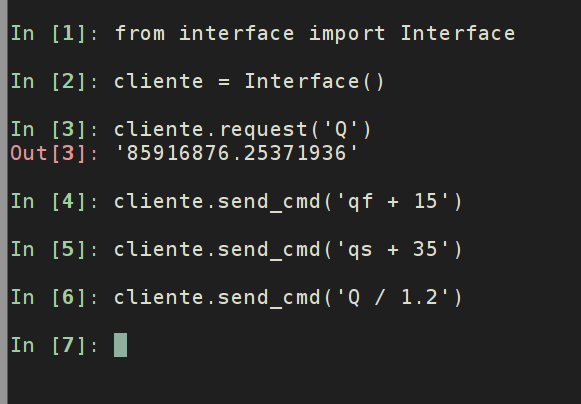
\includegraphics[scale=.25]{img/viewer_zoeira_console.png}}
  \subbottom[\label{pic_viewer_zoeira:viewer}Interface gráfica]{
    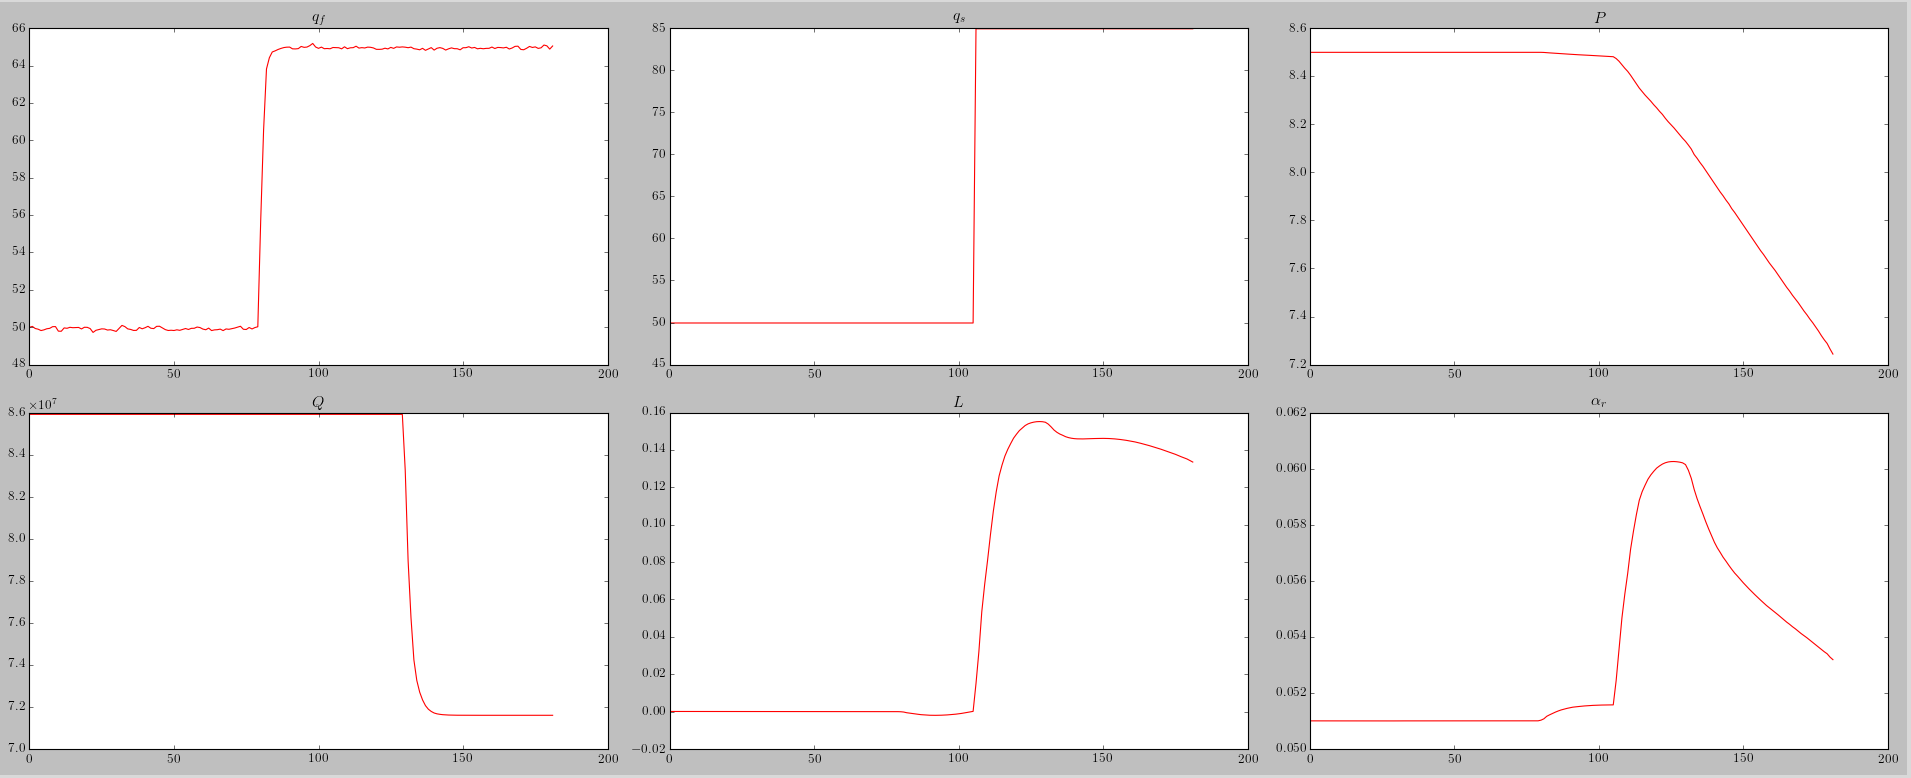
\includegraphics[scale=.25]{img/viewer_zoeira.png}}

\end{figure}

